\documentclass[letterpaper, 10 pt, conference]{ieeeconf}  
\IEEEoverridecommandlockouts                              % This command is only
                                                          % needed if you want to
                                                          % use the \thanks command
\overrideIEEEmargins
% See the \addtolength command later in the file to balance the column lengths
% on the last page of the document

% The following packages can be found on http:\\www.ctan.org
\usepackage{graphics} % for pdf, bitmapped graphics files
\usepackage{epsfig} % for postscript graphics files
\usepackage{amsmath} % assumes amsmath package installed
\usepackage{amssymb}  % assumes amsmath package installed
\usepackage{hyperref} %For hyperlinks
\usepackage{float} % To place graphs
\usepackage{epstopdf}
\usepackage{mathrsfs}


\title{\LARGE \bf
Recommendation Systems for Amazon.com
}
\author{Nikhil Johri, Zahan Malkani, and Ying Wang
}
\begin{document}

\maketitle
\thispagestyle{empty}
\pagestyle{empty}


%%%%%%%%%%%%%%%%%%%%%%%%%%%%%%%%%%%%%%%%%%%%%%%%%%%%%%%%%%%%%%%%%%%%%%%%%%%%%%%%
\begin{abstract}
Modern retailers frequently use recommendation systems to suggest products of 
interest to a collection of consumers. A closely related task is ratings 
prediction, in which the system predicts a numerical rating that a 
user $u$ will assign to a product $p$. In this paper, we build three ratings 
prediction models for a dataset of products and users from Amazon.com. We 
evaluate the strengths and weaknesses of each model, and discuss their 
effectiveness in a recommendation system.

\end{abstract}

%%%%%%%%%%%%%%%%%%%%%%%%%%%%%%%%%%%%%%%%%%%%%%%%%%%%%%%%%%%%%%%%%%%%%%%%%%%%%%%
\section{Introduction}
In this paper, we focus on collaborative filtering methods for recommendations. 
Collaborative filtering is the term applied to techniques that analyze the 
relationships between users and products in a large dataset and make 
recommendations based on existing connections between nodes \cite{bib:recsys}.
One common technique in collaborative filtering is to use existing connections 
to make judgments about similar products and users. Similarity depends only on 
history -- for example, two users may be similar if they have purchased many 
of the same items, so one user's rating can be used to infer a rating for 
another. 

The alternative to collaborative filtering is content filtering, which 
creates features for users and products to assess compatibility. These 
features, which in a book recommendation system might be things like genre or 
subject, will be scored for both users and products \cite{bib:recsys}. This 
makes content filtering highly domain-specific. 
In contrast, collaborative filtering does not need to create such features, 
so it is domain-independent. It is sufficient in collorative filtering to have 
only a matrix of users to products, where each entry in the matrix is some 
scalar indicator of the past relationship between a user and a product.

\subsection{Previous Work}
Collaborative filtering has enjoyed a long popularity in recommendations tasks. 
It was first used commercially in 1992 in a system called Tapestry to 
recommend newsgroup messages to readers \cite{bib:tapestry}. In this system, 
feedback and annotations from existing user-document relationships are used 
to select interesting documents for other users. This system first uses the 
term \emph{collaborative filtering} to indicate that people implicitly 
collaborate by recording their reactions to documents, enabling 
others to make decisions based on those reactions.

Our work is based on two broad categories of collaborative filtering: 
similarity methods and matrix factorization \cite{bib:recsys2}. Similarity 
methods make recommendations by comparing the similarity between users or 
products. In a neighborhood-based similarity model, users are compared to each 
other to determine their nearest neighbors based on their histories. Then, to 
make a prediction for user $u$'s opinion on product $p$, the model looks at the 
opinions of the neighbors of $u$ regarding $p$. Another similarity model is the 
item-based model, which examines item similarity instead of user similarity. 
This approach has been the basis for Amazon's own recommendation engine
 \cite{bib:amazon}. Its advantage is that product similarities can be computed 
offline, and when a user needs a product recommendation, the system performs 
a fast lookup of items similar to ones in the user's history . This speed 
has been beneficial for scalability in Amazon's large purchase network. 

The second type of collaborative filtering is model-based methods, in our case, 
matrix factorization. Matrix factorization does not use history to  model 
similarity like the previously discussed models. Instead, it uses past ratings 
to estimate the parameters of a statistical model for user-product 
relationships \cite{bib:matrixfact}. Users and products are represented as 
vectors in a latent vector space $R^f$. A numerical estimate for the 
opinion of  user $u$ on product $p$ can be obtained by taking the 
cross product of vectors for $u$ and $p$. The values of the latent dimensions 
are learned during a training stage by minimizing the error between known and 
predicted ratings.

Modern recommendation systems are often a combination of 
collaborative filtering, content-based filtering, and matrix factorization. 
One way to create a hybrid model is simply to take the outcomes of several 
approaches and merge them by taking a weighted average. Other 
hybrid techniques incorporate the previously discussed models with other
machine learning methods, such as classification \cite{bib:recsys2}. 
The ways to combine the approaches are numerous, and it is common for 
a recommendation system to incorporate a large number of strategies. 
The top entrants in the Netflix Prize used a hybrid algorithm with over 100 
techniques \cite{bib:bellkor}.

\subsection{Our project}
This project explores some of the most popular ratings prediction methods using 
a dataset from Amazon.com. The dataset, described in Section 
\ref{sec:dataset}, contains product purchase metadata of over 500,000 DVDs, 
music albums, books, and videos. We use both neighborhood-based and 
matrix factorization methods, described in Section \ref{sec:models}, and we 
discuss our findings in in Section \ref{sec:results}. Based on our 
experiments, we hope to shed some light on the nature of the recommendation 
task and the strengths of each of the models.


%%%%%%%%%%%%%%%%%%%%%%%%%%%%%%%%%%%%%%%%%%%%%%%%%%%%%%%%%%%%%%%%%%%%%%%%%%%%%%%
\section{Dataset}
\label{sec:dataset}
Our data comes from a collection of Amazon product purchase metadata from 
the Stanford Large Network Dataset Collection. The dataset contains over 
500,000 product entitities, including product title, salesrank, and ratings 
information. For our project, we are concerned with the ratings assigned 
by users to products. We parsed the dataset to a bipartite review 
graph whose nodes are products and users and edges are the ratings given by 
users to products. After extracting only the relevant data, we found many 
duplicate entries where a user $u$ has reviewed a product $p$ several times, 
sometimes assigning different ratings each time. After eliminating the 
duplicates, we reached a dataset with properties shown in 
Table~\ref{table:dataset}.



\begin{figure}[h]
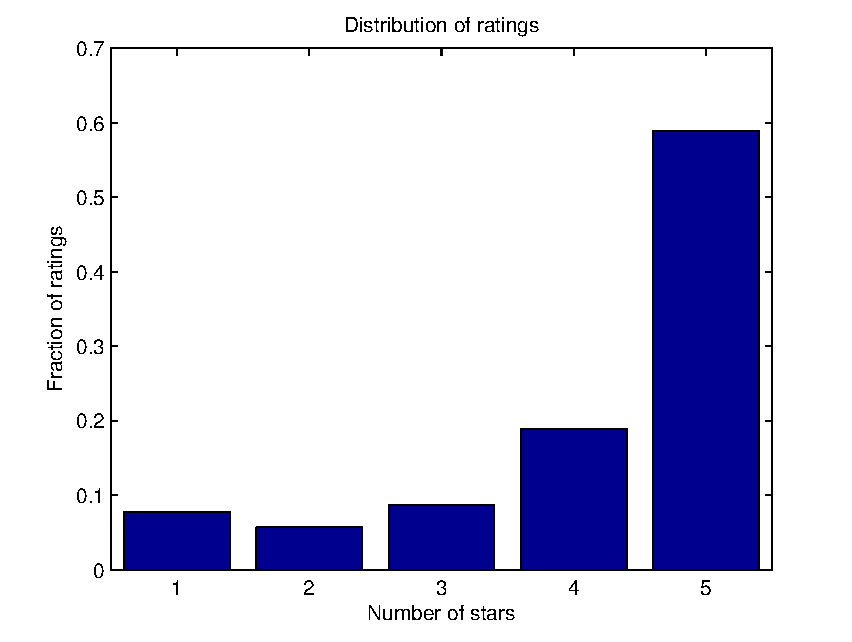
\includegraphics[scale=0.6]{images/ratings.pdf}
\caption{Star rating distribution}
\label{fig:ratings}
\end{figure}

\begin{figure}[h]
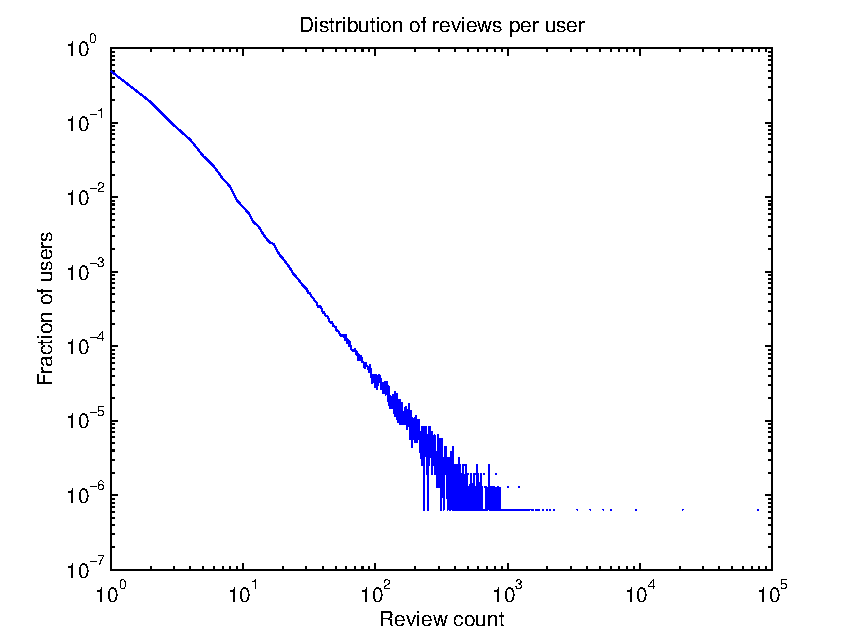
\includegraphics[scale=0.6]{images/user_hist.pdf}
\caption{User review count distribution}
\label{fig:userhist}
\end{figure}

\begin{figure}[h]
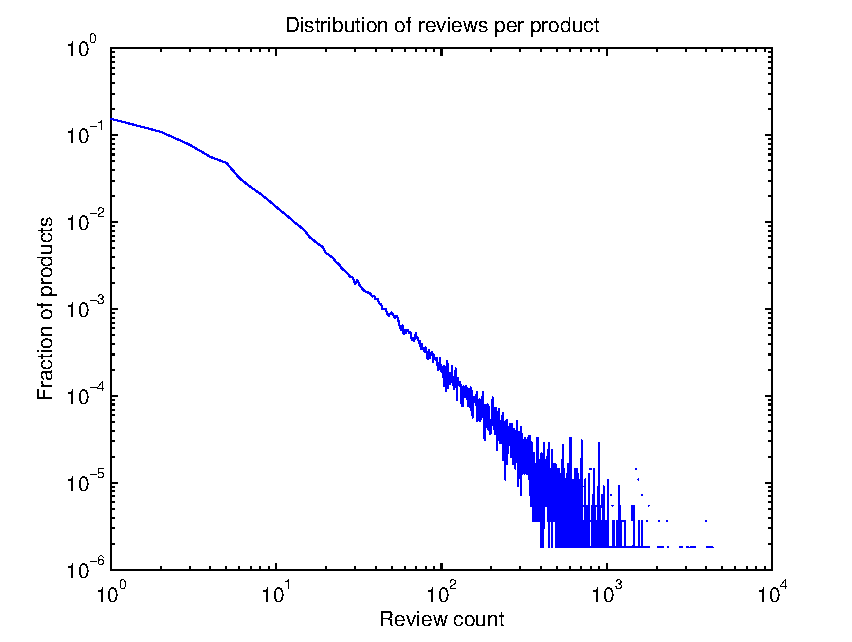
\includegraphics[scale=0.6]{images/product_hist.pdf}
\caption{Product review count distribution}
\label{fig:producthist}
\end{figure}

%%%%%%%%%%%%%%%%%%%%%%%%%%%%%%%%%%%%%%%%%%%%%%%%%%%%%%%%%%%%%%%%%%%%%%%%%%%%%%%
\section{Models}
\label{sec:models}

We plan to model the star rating a given user would assign to a given
venue or product. To begin, we will model our training data as a bipartite
graph, where each user is connected to an item if the user has reviewed
that item. The weight of the edge is the star count associated with that
review. The goal of our model is that for a (user, item) tuple without an
existing review, we will be able to predict the strength of the missing
edge.

We implemented three collaborative filtering algorithms on our dataset to
solve this problem of modified bipartite graph inference described
previously. Our first model, the neighborhood-based collaborative
filtering approach, focuses on similarity between users. The second model
we attempted was item-based collaborative filtering, which aims to utilize
similarity among products rated by the same user. Finally, our third model
assumes a hidden similarity layer exists between users and items, and
attempts to learn this using stochastic gradient descent. Further details
about these models are outlined below.

\subsection{Neighborhood-based model}

In this algorithm, we predict ratings for a user based on the known
ratings from similar users. The steps are outlined below:

\begin{enumerate}
  \item For a given user i, calculate similarity between this users and all
    other users. 
  \item Represent the dataset as a sparse matrix of businesses and users, with
    values in the matrix being the ratings assigned by the users to the
    businesses. Take the cosine similarity between the vectors of two users.
  \item Select the k nearest neighbors of i based on this similarity measure
  \item Compute a predicted rating for i based on a weighted combination of the
    nearest neighbors. ratings
\end{enumerate}

We tried our model on both the original datasets (for both Yelp and
Amazon), as well as a pruned Amazon dataset that included only users that
had a minimum of 5 reviews and items with a minimum of 5 reviewers. While
running this model on the un-pruned datasets, we found a number of
instances where our test user would have only a single review (which we
would be trying to predict), rendering the algorithm useless. Such
examples were removed from our test set. 

\subsection{Modified neighborhood model}

Given the sparsity of our datasets, we decided to try a variation of the
neighborhood based collaborative filtering approach, in which, instead of
simply selecting the k nearest neighbors for a user, we select the k
nearest neighbors out of those who have rated the product. This works
poorly for items that have fewer than k reviews, as we end up simply
calculating the average of the scores assigned to those items. However, we
found that this modification worked very well in our high activity
dataset, as there was enough information for each user and each item to
make an informed decision. 

\subsection{Item-based model}

In their work on item-base collaborative filtering algorithms,
\cite{bib:sarwar} take a different approach to the nearest
neighbor problem, focusing on the similarities between items rather than
users. In a similar vein, we will use the graph structure in the bipartite
graph of users and businesses to compute a similarity metric between
businesses. The motivating intuition being that users are likely to rate
similar businesses comparably, yielding a better prediction for the (user,
business) pair than the neighborhood-based method.

Considering the item-space rather than the user space takes care of a few
crucial problems. Namely, the search for similar users in the
high-dimensional space of user profiles over the large set of all Yelp.s
users is prohibitively computationally expensive. It also partially takes
into account a missing data problem regarding new profiles which have
comparatively few ratings for businesses.

The steps involved in item-based collaborative filtering are as follows:
\begin{enumerate}
\item When considering the (user, item) pair, calculate similarities between
  the target business and each of the items the user has rated previously
\item Use cosine similarity and use all of the ratings for a particular item
  over the user space as the feature vector to measure similarity between
  items.
\item Look for the k nearest neighbors to the target item from among the set of
  items the user has rated previously
\item Take a weighted average of the selected k items to compute a prediction
  of the rating for the target item
\end{enumerate}

Once again, we encountered similar situations as described in the
neighborhood-based collaborative filtering approach when evaluating our
model on the un-pruned datasets, caused by the sparsity of the data. We
removed (user, item) test cases in which the user had only a single review
or the item had only one reviewer when testing.

\subsection{Matrix factorization}

In our final model, we aim to predict ratings by estimating
parameters for statistical models for user ratings. Unlike the previous
two methods which projected user ratings based on user similarity or
item similarity, matrix factorization models assume that a similarity layer
between users and items is induced by a hidden lower-dimensional structure
latently present in the data.

If we associate each item $i$ with a vector $q_i \in R^f$, and each user $u$ with a
vector $p_u \in R^f$, then we can use the resulting dot product $q_i^Tp_u$ to represent
the interest between user $u$ and item $i$. The problem then turns into a
learning problem where we attempt to learn the distribution vectors for
$q_i,p_u$. 

A number of methods can be employed to learn these factor vectors for
users and items. In their work on Netflix recommender systems,
\cite{bib:bellkor} describe possible usage of two common approaches, namely,
stochastic gradient descent and alternating least squares. Given the
sparsity of our training set, stochastic gradient descent was a suitable
option, whereby we computed, at each step, a prediction error $e_{ui}
=r_{ui}-q_i^Tp_u$ for each user-item training pair, and adjust our
parameters $q_i,p_u$ accordingly in the opposite direction of the gradient.


%%%%%%%%%%%%%%%%%%%%%%%%%%%%%%%%%%%%%%%%%%%%%%%%%%%%%%%%%%%%%%%%%%%%%%%%%%%%%%%
\section{Results and Discussion}
\label{sec:results}

We report the results of our models on the full Amazon dataset and on our 
high-activity subset. We measure performance over the test sets using 
root-mean-square error. The errors are normalized by dividing by 4, the maximum 
difference between the highest and lowest star ratings possible. However, 
in the interest of preserving granularity for model comparison, predicted
fractional ratings are not rounded to the nearest integer before calculating 
the errors. 

\subsection{Neighborhood-based model}
\subsubsection{Full dataset}
The results of the neighborhood-based model on the full dataset are shown in 
table ?? and Figure ?? below.


\begin{table}[htb]
\centering
\begin{tabular}{|c|c|c|}
\cline{2-3}

\multicolumn{1}{c|}{} & \vbox{\hbox{\strut Neighborhood model}} 
& \vbox{\hbox{\strut Modified }\hbox{\strut neighborhood model}} \tabularnewline \hline
$k$ = 1 & 0.3497 & 0.3870 \tabularnewline
$k$ = 3 &  0.3374 & 0.3544 \tabularnewline
$k$ = 5 & 0.3348 & 0.3448 \tabularnewline
$k$ = 10 & 0.3262 & 0.3397 \tabularnewline
$k$ = 25  & 0.3220 & 0.3346 \tabularnewline
\hline
All other users & \multicolumn{2}{|c|}{?}  \tabularnewline
\hline
Always predict 4 & \multicolumn{2}{|c|}{0.3211}  \tabularnewline
\hline
\end{tabular}
\caption{Neighborhood models, full dataset}
\end{table}

\subsubsection{High-activity dataset}

\begin{table}[htb]
\centering
\begin{tabular}{|c|c|c|}
\cline{2-3}

\multicolumn{1}{c|}{} & \vbox{\hbox{\strut Neighborhood model}} 
& \vbox{\hbox{\strut Modified }\hbox{\strut neighborhood model}} \tabularnewline \hline
$k$ = 1 &  & 0.1397 \tabularnewline
$k$ = 3 &  & 0.1864 \tabularnewline
$k$ = 5 &  & 0.2180 \tabularnewline
$k$ = 10 & & 0.2493 \tabularnewline
$k$ = 25  &  & 0.2645 \tabularnewline
\hline
All other users & \multicolumn{2}{|c|}{}  \tabularnewline
\hline
Always predict 4 & \multicolumn{2}{|c|}{0.3039}  \tabularnewline
\hline
\end{tabular}
\caption{Neighborhood models, full dataset}
\end{table}


\subsection{Item-based model}
\subsection{Matrix factorization}

%%%%%%%%%%%%%%%%%%%%%%%%%%%%%%%%%%%%%%%%%%%%%%%%%%%%%%%%%%%%%%%%%%%%%%%%%%%%%%%
\section{Conclusion}


\begin{thebibliography}{99}

\bibitem{bib:recsys}
Adomavicius, G., Tuzhilin, A. (2005). Toward the next generation of recommender systems: a survey of the state-of-the-art and possible extensions. Knowledge and Data Engineering, IEEE Transactions on , 17(6),  734- 749.

\bibitem{bib:matrixfact}
Bell, R., Koren, Y., Volinsky, C. (2009). Matrix factorization techniques for recommender systems. IEEE Computer 42(8):30-37

\bibitem{bib:bellkor}
Bell, R., Koren, Y., Volinsky, C. (2009). 
The BellKor solution to the Netflix Prize. Technical Report, AT\&T Labs 
Research, 2007b. 
http://www.netflixprize.com/assets/ProgressPrize2007\_KorBell.pdf


\bibitem{bib:tapestry}
Goldberg, D., Nichols, D., Oki, B., Terry, D. (1992). 
Using collaborative filtering to weave an information tapestry. 
Communications of the Association of Computing Machinery, 35(12), 61-70.

\bibitem{bib:amazon}
Linden, G., Smith, B., York, J. (2003). Amazon.com recommendations: Item-to-item collaborative filtering. IEEE Internet
Computing, 7(1), 76-80.

\bibitem{bib:recsys2}
Melville, P., Sindhwani, V. (2010).
Recommender Systems. The Encyclopedia of Machine Learning. 
http://www.prem-melville.com/publications/recommender-systems-eml2010.pdf

\bibitem{bib:sarwar}
Badrul Sarwar, George Karypis, Joseph Konstan, and John Reidl. 2001.
Item-based collaborative filtering recommendation algorithms.
In Proceedings of the 10th international conference on World Wide Web (WWW '01). ACM, New York, NY, USA, 285-295. 

\end{thebibliography}

\end{document}
